	
In these experiments, several current techniques (2D Feature Matching (FM-2D), 3D Feature Matching (FM-3D), ICP and PCA) are compared to the FVR technique in terms of stereo camera registration accuracy. To this end, five data sets from the Kitti Vision Benchmark data set \cite{Geiger13Vision} were used. Each data set scene is a complicated outdoor environment filmed using an autonomous driving platform. The majority of frames contain moving objects which interfere with the registration process of several algorithms. \\

Each Kitti Vision Benchmark data set contains accurate laser scans, stereo grey-scale images, stereo RGB-images and GPS and IMU data. To simulate the theoretical situation in which stereo cameras generate the most accurate depth maps, the laser scans are used in place of depth data computed by a stereo disparity algorithm. Therefore, in these experiments, only the laser scans and stereo colour and greyscale images are used. \\

The five stereo data sets used in the experiments are shown in Figures \ref{fig:KT1DSS}, \ref{fig:KT2DSS}, \ref{fig:KT5DSS}, \ref{fig:KT91DSS} and \ref{fig:KT95DSS}. The first scene is the Kitti 0001 Sync Data Set, this scene has 107 frames. This data set contains 12 cars, two cyclists and a tram. The tram and cyclists are non-static objects within the scene, making it more difficult for the current set of reconstruction algorithms which rely on scenes being primarily static in nature. To the right in this data set, there is a tram-line and some trees and gardens, to the left is a residential street. The second scene is the Kitti 0002 Sync data set, this set is 76 frames long. It contains one car and two cyclists which are non-static objects. Within this scene there is a long brick wall hiding some tall trees, several cyclists ride along next to the wall. To the left, there are some grassy areas, some buildings and some parked cars. \\

At 153 frames, the Kitti 0005 Sync data set is also used. This scene contains nine cars, three vans, two pedestrians and one cyclist. Because of the size of the van and the other non-static objects within the scene, this appears to be one of the more difficult scenes to register. The camera winds through several different streets as opposed to the previous data sets which are mostly of one long road. The fourth data set used, the Kitti 0091 Sync data set is composed of 339 frames making it the largest data set used in these experiments. This data set contains two cars, a van, 42 pedestrians, 14 sitters, eight cyclists and one miscellaneous object. As it contains many non-static objects this scene is also considered difficult like the Kitti 0005 data set. \\

The last Kitti Vision Benchmark data set used is the Kitti 0095 data set. Unlike the previous data sets, all 267 frames only contain static objects, and the scenes are made up primarily of small winding streets. \\ 

Experiments are tabled in full at per frame intervals in Appendix \ref{StereoResultsRaw}. Here, registration errors are presented where frame $n$ is registered against frame $n+1$ and the registration error is reported for each algorithm. The error function used is the Mean Squared Error $MSE(P,Q)$. This error is computed between the consecutive frames after registration. This error value is computed as in equation \ref{eqn:msesota}. Here, the function $Register(x)$ is replaced by the registration method being tested. \\

\begin{equation} \label{eqn:msesota}
Error(frame_1, frame_2) =  \frac{Register(frame_1), frame2}{MSE(frame_1,frame_2)}
\end{equation}

\begin{figure*}[t]
\centering
\begin{subfigure}[b]{1.5in}
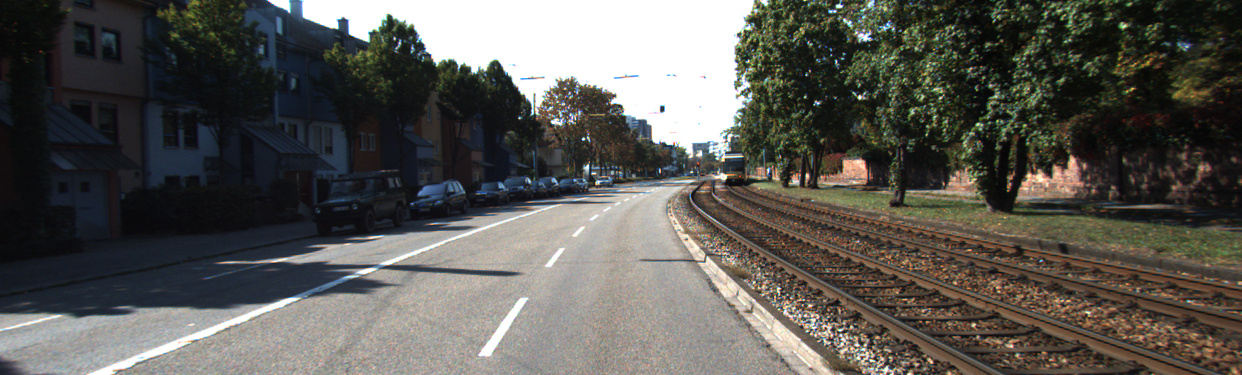
\includegraphics[width=1.5in]{{images/experiments/stereo/1.1}.png}
\caption{Frame 1}
\end{subfigure}%
\begin{subfigure}[b]{1.5in}
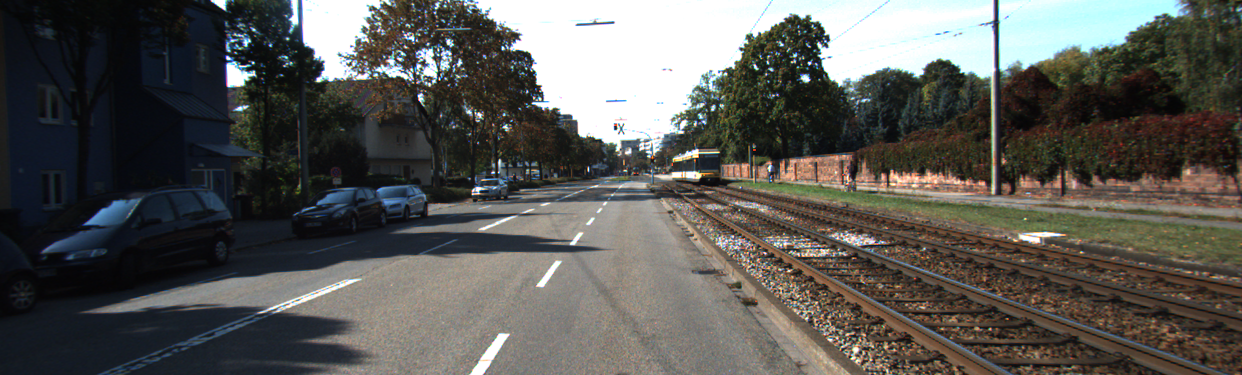
\includegraphics[width=1.5in]{{images/experiments/stereo/1.2}.png}
\caption{Frame 39}
\end{subfigure}%
\begin{subfigure}[b]{1.5in}
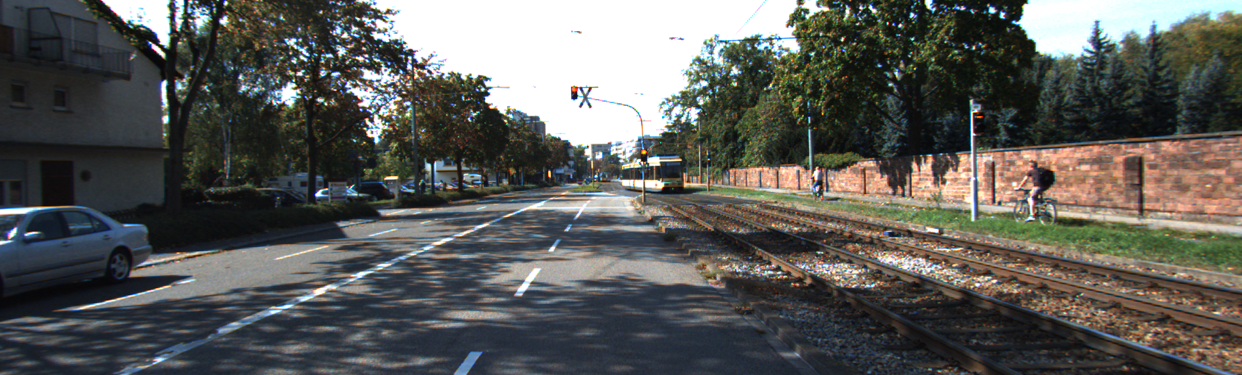
\includegraphics[width=1.5in]{{images/experiments/stereo/1.3}.png}
\caption{Frame 77}
\end{subfigure}%
\begin{subfigure}[b]{1.5in}
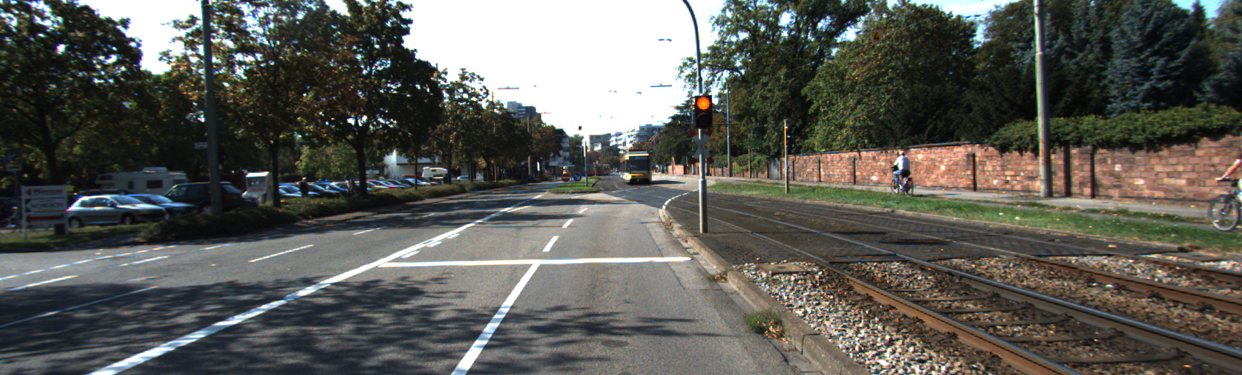
\includegraphics[width=1.5in]{{images/experiments/stereo/1.4}.png}
\caption{Frame 114}
\end{subfigure}%
\caption{Kitti 0001 Sync Data Set Sample}
\label{fig:KT1DSS}
\end{figure*}


The summary of these results is also tabled here for convenience. For each algorithm, the median registration error is provided. This is computed by listing and sorting the registration error values for a particular algorithm and selecting the value in the middle. Also included is the percent of best results metric. This measures in percentage, the frequency of times a particular algorithm achieved the best (lowest error) registration result compared to the other algorithms tested. An algorithm with a lower median error than another algorithm has performed better overall. Additionally, if an algorithm has a higher percentage of best results, it outperformed the other algorithms most of the time. If an algorithm achieved an average percentage of best results but a higher median error, this could be explained by outliers. If an algorithm achieved a lower median error but did not achieve the highest percentage of best results, it may be due to having a very competitive and consistent registration error. \\


Table \ref{tab:kittidata0001sync} presents results for the Kitti 0001 Sync data set, some example colour frames are shown in Figure \ref{fig:KT1DSS}. The road in which this scene was filmed contains a tram-line and moving tram as well as a garden area to the right and a line of parked cars and houses under cover of shadows to the left. Registration statistics were taken over the full length of this data set, which is 107 frames. Results show that FVR-3D achieved the lowest median registration error, ICP achieved the next lowest followed by FM2D and the FVR method. FVR-3D also achieved the highest percentage of best frame registration results at ~34.91 \% compared to ICP with ~27.36 \%. If the FVR methods were combined as a single hybrid method, they would have computed the best registration result 55.67 \% of the time. The FVR method alone outperformed FFVR, PCA and FM-3D. The FM-3D method (which had several frame registration failures, as is evident in its statistics) and the PCA method were the worst performers on this data set. The FFVR, whilst faster than the FVR method is slightly worse off in terms of performance. \\ 

%% sync 0001
\begin{table}[t]
\centering
\caption{Reconstruction Errors for the Kitti Data 0001 Sync Data Set}
\begin{tabular}{ccc}
\hline
\textbf{Algorithm} & \textbf{Median Error $\times$ 1000} & \textbf{\% best results}\\ \hline
FM2D	& 5.28 & 13.21\%\\
FM3D	& 9235.71 & 0.94\%\\
ICP	& 5.15 & 27.36\%\\
PCA	& 5.66 & 2.83\%\\
FVR	& 5.5 & 13.21\%\\
FFVR	& 5.59 & 7.55\%\\
FVR-3D	& 5.1 & 34.91\%\\
\end{tabular}
\label{tab:kittidata0001sync}
\end{table}








Table \ref{tab:kittidata0002sync} presents median error and percent best result statistics for the Kitti 0002 Sync Data Set, example colour frames are shown in Figure \ref{fig:KT2DSS}. The road in which this scene contains some parked cars to the left as well as a building, some grass and some large trees. To the right there is an orange brick wall and some trees and gardens as well as two moving cyclists. Results for the full 74 frames of the data set show that the FVR-3D method achieved the lowest median registration error at 4.27. The ICP algorithm achieved the next best result at 4.43 and the non-rotation-invariant FVR method achieved the third best result. Combined, the FVR based methods achieved the best result ~50.67 \% of the time compared to ICP at 30.67 \%. In this scene, the FM-3D method did not have as many registration failures and achieved a better result than the FFVR method and a comparable result to the PCA method. \\ 

%% sync 0002
\begin{table}[t]
\centering
\caption{Reconstruction Errors for the Kitti Data 0002 Sync Data Set}
\begin{tabular}{ccc}
\hline
\textbf{Algorithm} & \textbf{Median Error $\times$ 1000} & \textbf{\% best results}\\ \hline
FM2D	& 4.78 & 5.33\%\\
FM3D	& 4.85 & 6.67\%\\
ICP	& 4.43 & 30.67\%\\
PCA	& 4.86 & 6.67\%\\
FVR	& 4.67 & 6.67\%\\
FFVR	& 5.23 & 5.33\%\\
FVR-3D	& 4.27 & 38.67\%\\
\end{tabular}
\label{tab:kittidata0002sync}
\end{table} 



\begin{figure*}[t]
\centering
\begin{subfigure}[b]{1.5in}
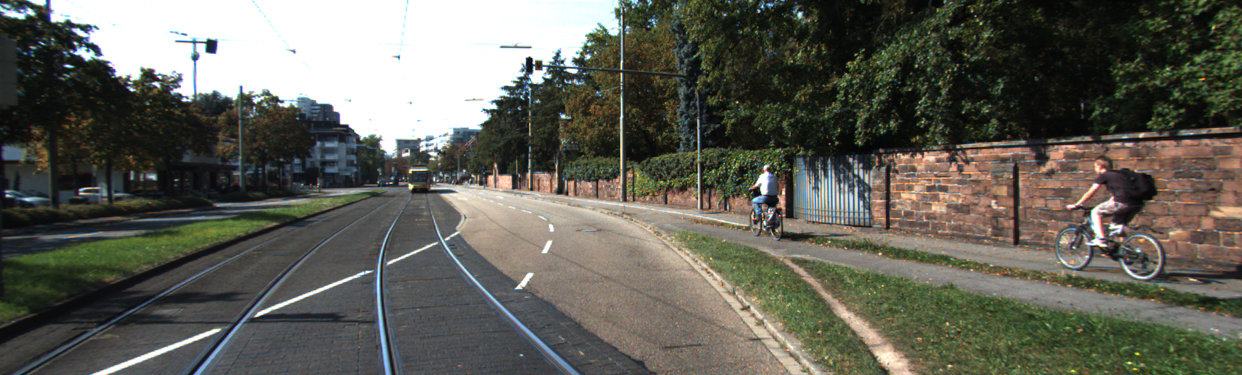
\includegraphics[width=1.5in]{{images/experiments/stereo/2.1}.png}
\caption{Frame 1}
\end{subfigure}%
\begin{subfigure}[b]{1.5in}
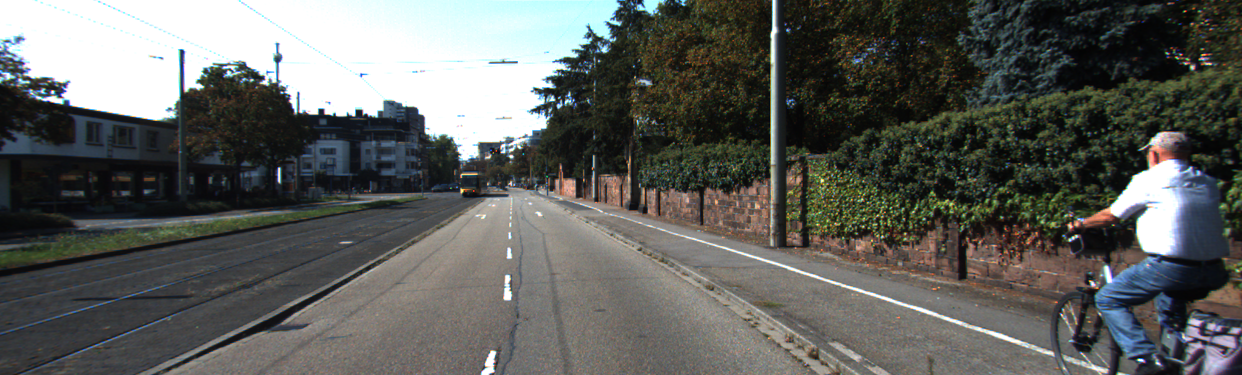
\includegraphics[width=1.5in]{{images/experiments/stereo/2.2}.png}
\caption{Frame 28}
\end{subfigure}%
\begin{subfigure}[b]{1.5in}
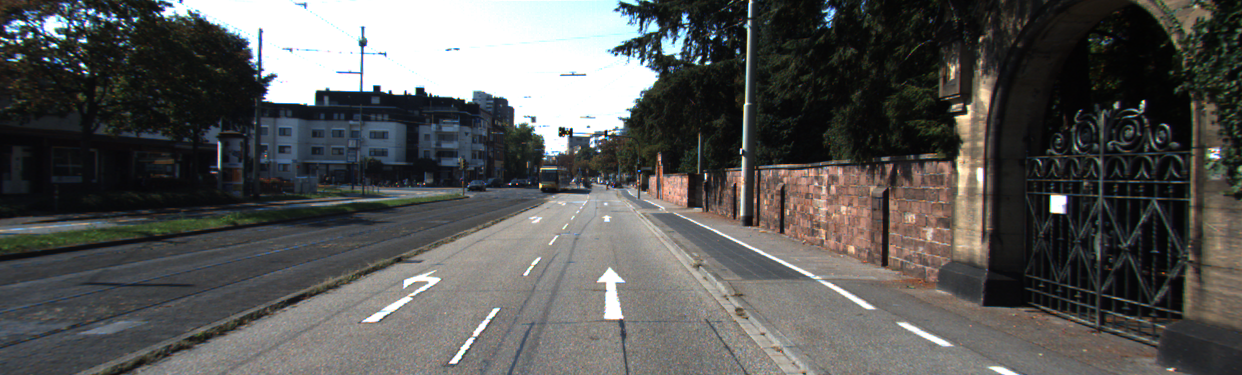
\includegraphics[width=1.5in]{{images/experiments/stereo/2.3}.png}
\caption{Frame 56}
\end{subfigure}%
\begin{subfigure}[b]{1.5in}
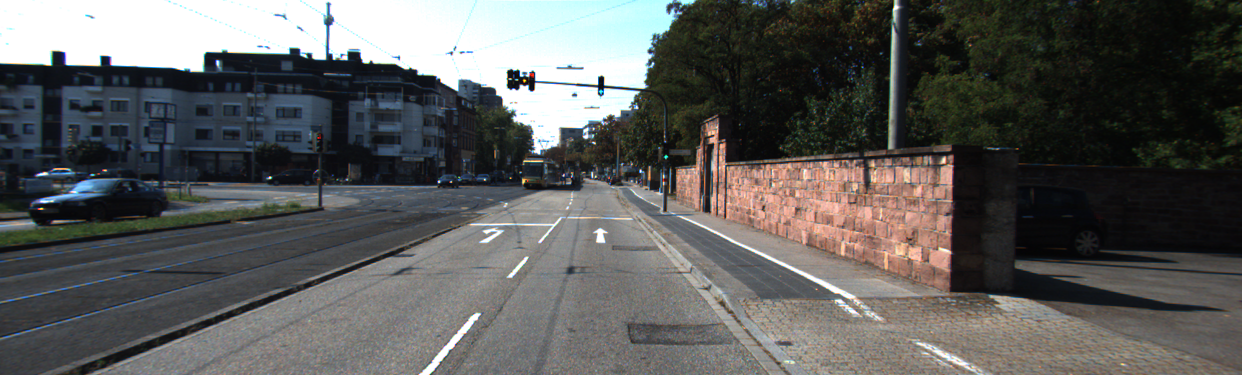
\includegraphics[width=1.5in]{{images/experiments/stereo/2.4}.png}
\caption{Frame 83}
\end{subfigure}%
\caption{Kitti 0002 Sync Data Set Sample}
\label{fig:KT2DSS}
\end{figure*}



 

Statistics for the Kitti 0005 Sync Data Set are presented in Table \ref{tab:kittidata0005sync}, example colour frames are shown in Figure \ref{fig:KT5DSS}. The scene captured in this data set was more difficult than previous scenes as it contains two moving cyclists and one large van which are all moving around in the scene without any relation to camera movement. In other words, these non-static objects cause major difficulties in most registration algorithms. In the full 152 frames of the data set, FM2D performed best with the lowest median error and highest percentage of best results. Next, FVR-3D also performed well with the second best median error and percentage of best results measurement. ICP achieved the third best median error and percentage of best results. In the results for this data set, FVR outperformed the FFVR method, as well as PCA and FM3D. Combined, the FVR algorithms achieved the best registration result 35.29 \% of the time, which is still below the performance of FM2D on this data set. \\

%% 0005
\begin{table}[t]
\centering
\caption{Reconstruction Errors for the Kitti Data 0005 Sync Data Set}
\begin{tabular}{ccc}
\hline
\textbf{Algorithm} & \textbf{Median Error $\times$ 1000} & \textbf{\% best results}\\ \hline
FM2D	& 3.39 & 39.22\%\\
FM3D	& 3.83 & 0\%\\
ICP	& 3.49 & 25.49\%\\
PCA	& 4.06 & 0\%\\
FVR	& 3.7 & 5.88\%\\
FFVR	& 4.25 & 1.96\%\\
FVR-3D	& 3.42 & 27.45\%\\
\end{tabular}
\label{tab:kittidata0005sync}
\end{table}

\begin{figure*}[t]
\centering
\begin{subfigure}[b]{1.5in}
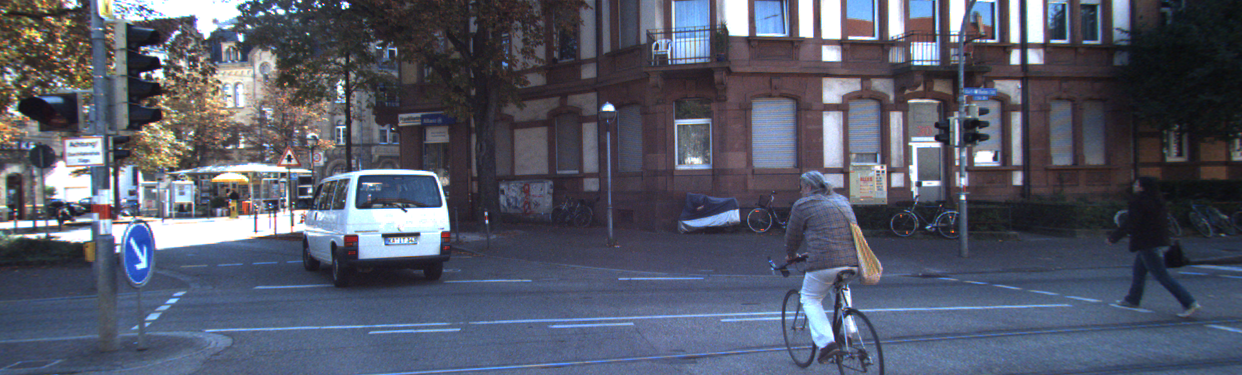
\includegraphics[width=1.5in]{{images/experiments/stereo/5.1}.png}
\caption{Frame 1}
\end{subfigure}%
\begin{subfigure}[b]{1.5in}
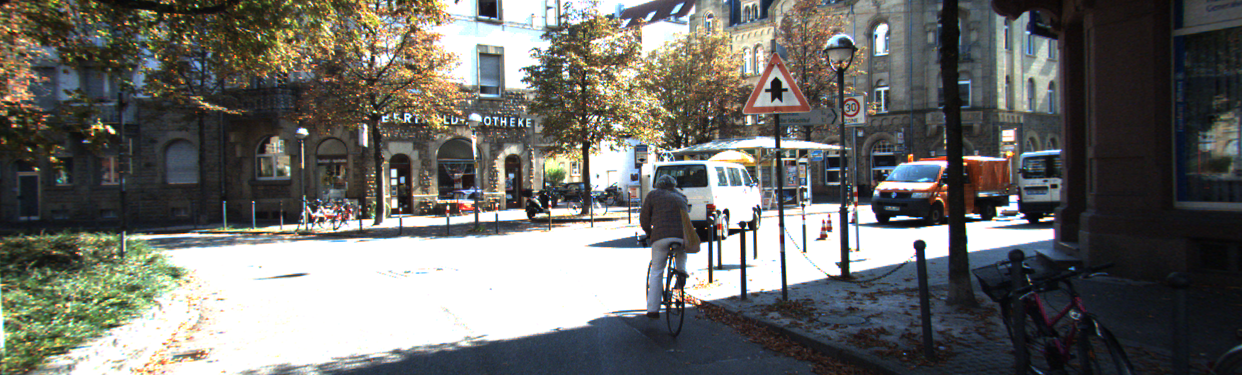
\includegraphics[width=1.5in]{{images/experiments/stereo/5.2}.png}
\caption{Frame 54}
\end{subfigure}%
\begin{subfigure}[b]{1.5in}
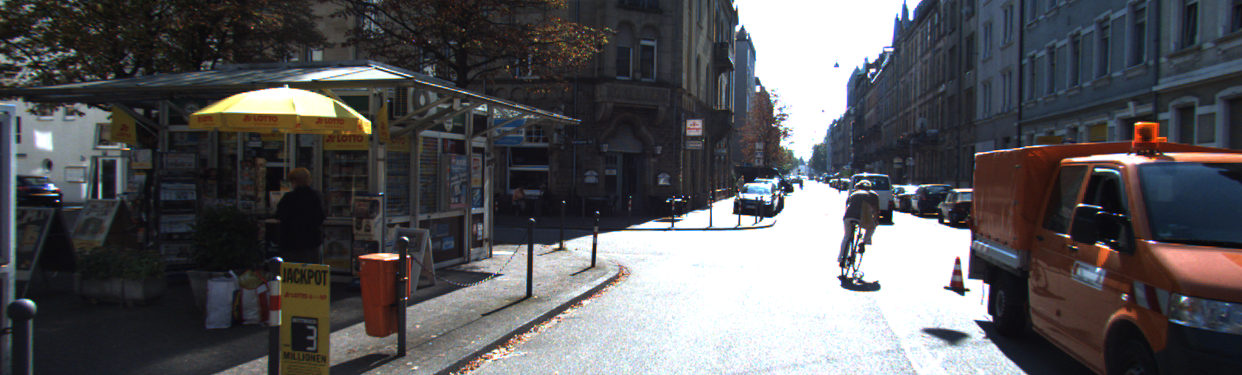
\includegraphics[width=1.5in]{{images/experiments/stereo/5.3}.png}
\caption{Frame 107}
\end{subfigure}%
\begin{subfigure}[b]{1.5in}
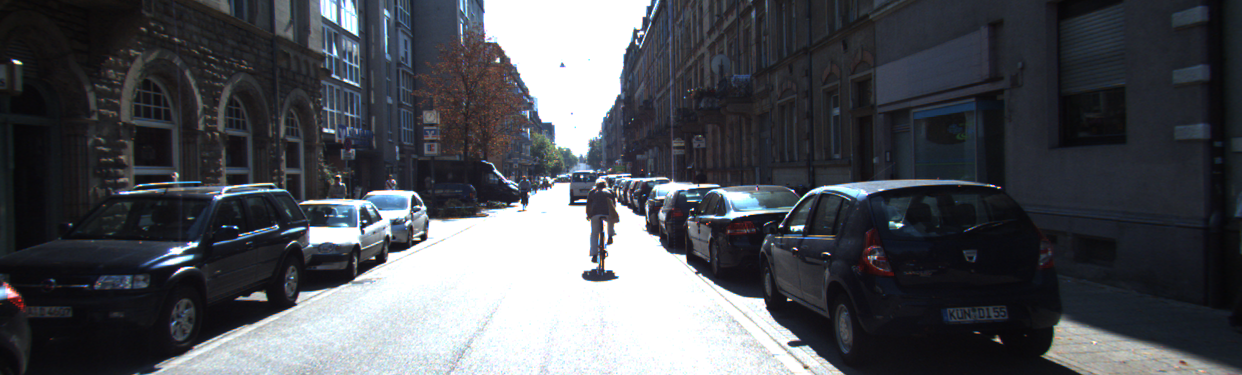
\includegraphics[width=1.5in]{{images/experiments/stereo/5.4}.png}
\caption{Frame 160}
\end{subfigure}%
\caption{Kitti 0005 Sync Data Set Sample}
\label{fig:KT5DSS}
\end{figure*}



Table \ref{tab:kittidata0091sync} presents results for the Kitti 0091 Data Set, example colour frames from the data set are shown in Figure \ref{fig:KT91DSS}. This is the largest data set tested at 339 frames. The scene filmed in this data set is that of an outdoors inner city. It contains many moving agents making it a scene which is difficult to register for most registrations algorithms. Specifically, it contains two cars, a van, 42 pedestrians and eight cyclists. Registration results show FVR-3D outperformed all the other algorithms in terms of both median error and percentage of best results. The FVR algorithm achieved the next best results. The FVR-3D algorithm achieves the best result more than twice as often as ICP and FM2D. The FVR based methods performed well on this data set, a hybrid approach would have achieved the best results 65.19 \% of the time.  \\  	

%% kitti dataset 0091 Sync
\begin{table}[t]
\centering
\caption{Reconstruction Errors for the Kitti Data 0091 Sync Data Set}
\begin{tabular}{ccc}
\hline
\textbf{Algorithm} & \textbf{Median Error $\times$ 1000} & \textbf{\% best results}\\ \hline
FM2D	& 3.6 & 17.11\%\\
FM3D	& 4.04 & 0.88\%\\
ICP	& 3.61 & 15.63\%\\
PCA	& 4.1 & 1.18\%\\
FVR	& 3.57 & 20.94\%\\
FFVR	& 3.78 & 5.9\%\\
FVR-3D	& 3.43 & 38.35\%\\
\end{tabular}
\label{tab:kittidata0091sync}
\end{table} 


\begin{figure*}[t]
\centering
\begin{subfigure}[b]{1.5in}
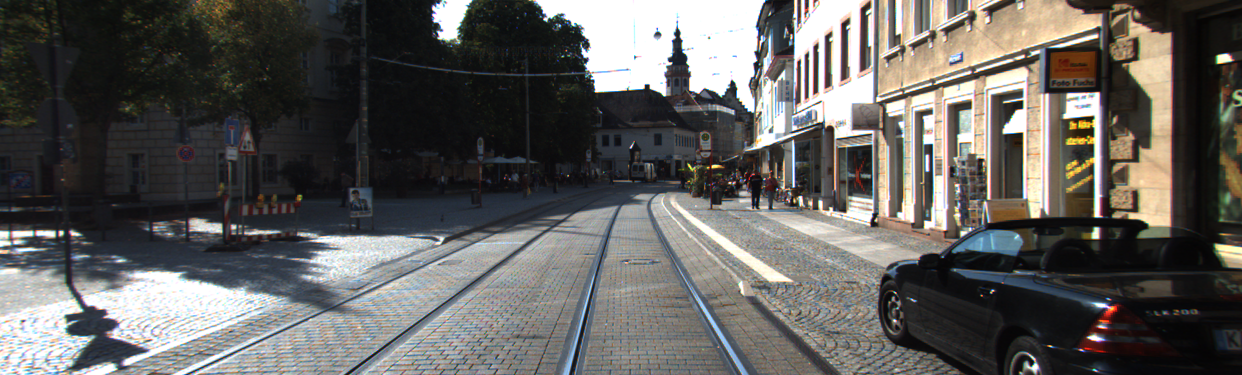
\includegraphics[width=1.5in]{{images/experiments/stereo/91.1}.png}
\caption{Frame 1}
\end{subfigure}%
\begin{subfigure}[b]{1.5in}
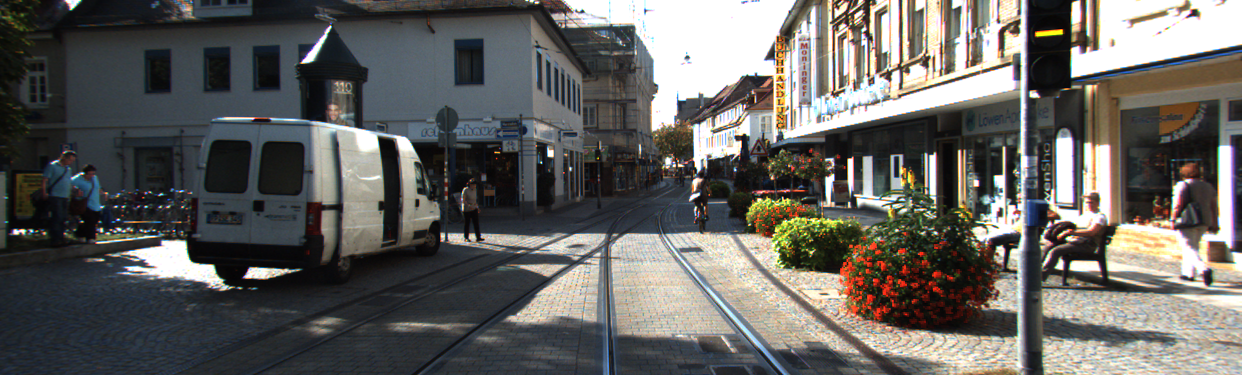
\includegraphics[width=1.5in]{{images/experiments/stereo/91.2}.png}
\caption{Frame 116}
\end{subfigure}%
\begin{subfigure}[b]{1.5in}
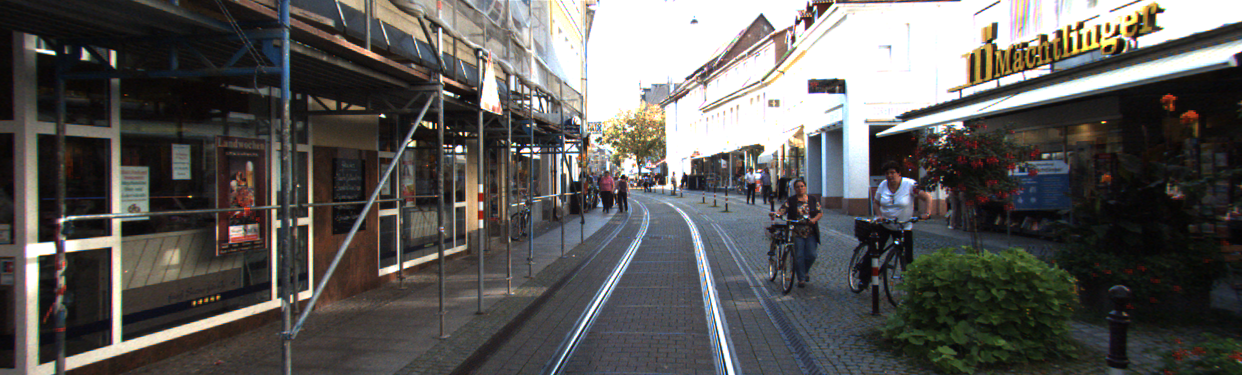
\includegraphics[width=1.5in]{{images/experiments/stereo/91.3}.png}
\caption{Frame 231}
\end{subfigure}%
\begin{subfigure}[b]{1.5in}
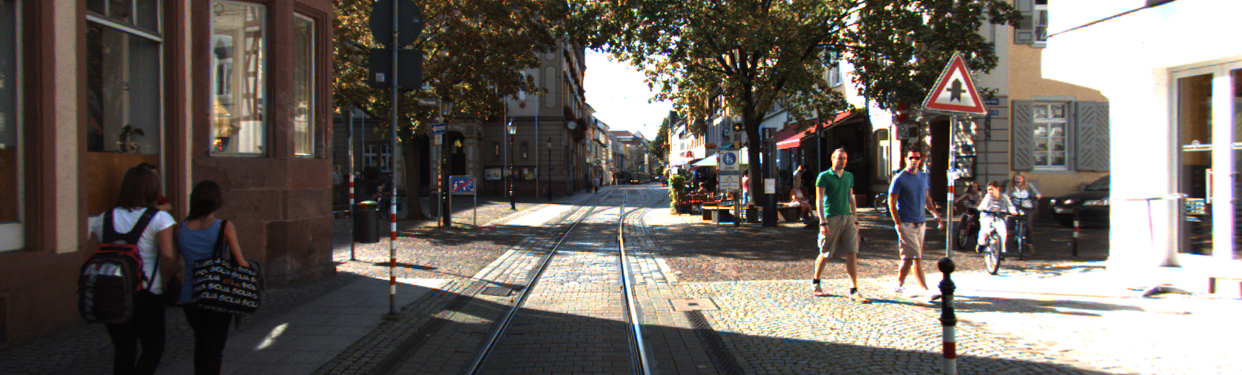
\includegraphics[width=1.5in]{{images/experiments/stereo/91.4}.png}
\caption{Frame 346}
\end{subfigure}%
\caption{Kitti 0091 Sync Data Set Sample}
\label{fig:KT91DSS}
\end{figure*}



Results for the Kitti 00095 Data Set are presented in Table \ref{tab:kittidata0095sync} and Figure \ref{fig:KT95DSS} presents four example colour images from this data set. This scene was much more static than the previous scenes. It contains primarily parked cars and buildings in an inner-city environment. There are a few pedestrians and cyclists which are moving agents within the scene. This data set is 266 frames and results show that FVR-3D achieves both the best (lowest) median error score and the highest percentage of best results score at ~46.82 \%. The FVR algorithm achieved the second best results in terms of both the median error and percentage of best results metrics. ICP and FM2D were third and fourth, respectively. The FVR-3D algorithm achieved the best result three times more often than both the ICP and FM2D methods. \\

%% sync 0095
\begin{table}[t]
\centering
\caption{Reconstruction Errors for the Kitti Data 0095 Sync Data Set}
\begin{tabular}{ccc}
\hline
\textbf{Algorithm} & \textbf{Median Error $\times$ 1000} & \textbf{\% best results}\\ \hline
FM2D	& 4.19 & 12.36\%\\
FM3D	& 5.18 & 0\%\\
ICP	& 4.4 & 13.48\%\\
PCA	& 5.32 & 0.37\%\\
FVR	& 4.12 & 22.85\%\\
FFVR	& 4.73 & 4.12\%\\
FVR-3D	& 3.96 & 46.82\%\\
\end{tabular}
\label{tab:kittidata0095sync}
\end{table} 


\begin{figure*}[t]
\centering
\begin{subfigure}[b]{1.5in}
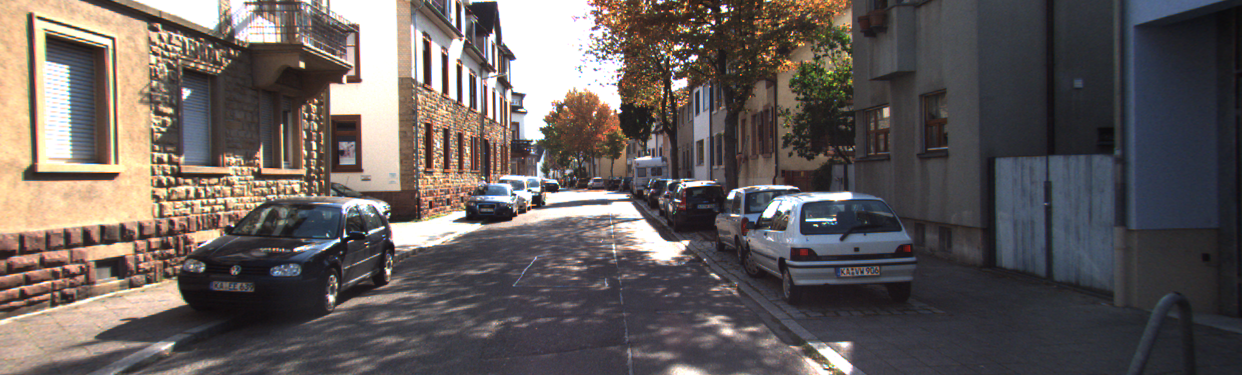
\includegraphics[width=1.5in]{{images/experiments/stereo/95.1}.png}
\caption{Frame 1}
\end{subfigure}%
\begin{subfigure}[b]{1.5in}
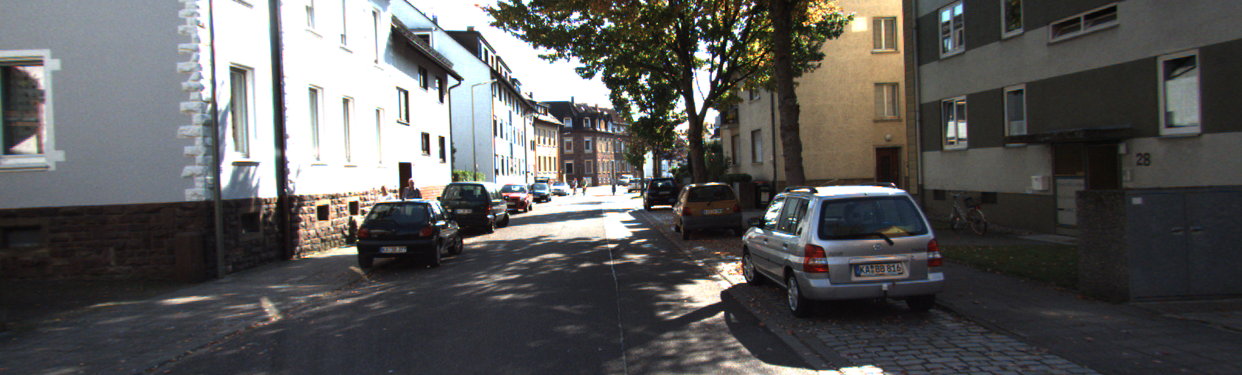
\includegraphics[width=1.5in]{{images/experiments/stereo/95.2}.png}
\caption{Frame 92}
\end{subfigure}%
\begin{subfigure}[b]{1.5in}
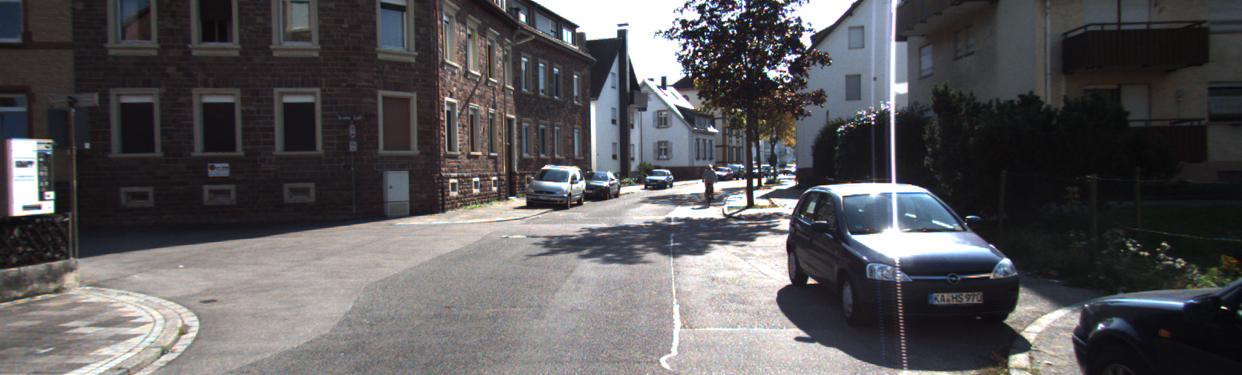
\includegraphics[width=1.5in]{{images/experiments/stereo/95.3}.png}
\caption{Frame 183}
\end{subfigure}%
\begin{subfigure}[b]{1.5in}
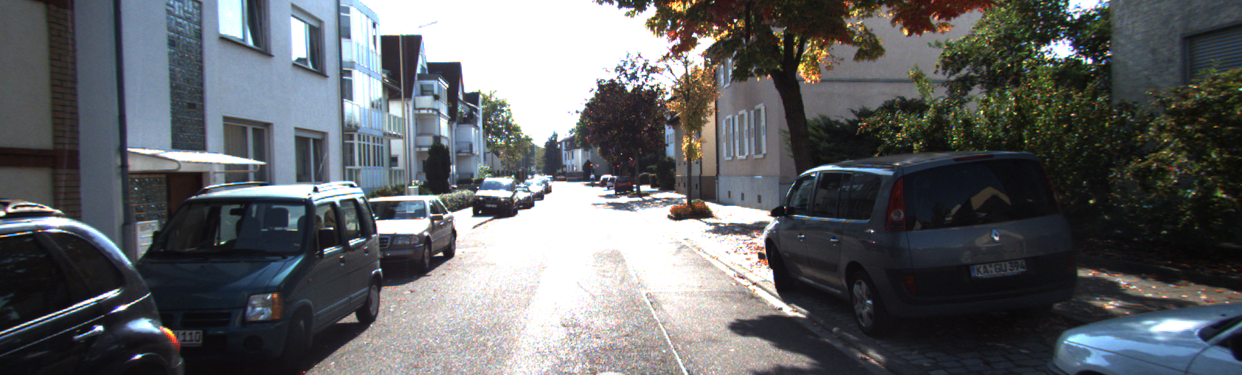
\includegraphics[width=1.5in]{{images/experiments/stereo/95.4}.png}
\caption{Frame 274}
\end{subfigure}%
\caption{Kitti 0095 Sync Data Set Sample}
\label{fig:KT95DSS}
\end{figure*}
